\documentclass{article}

%%%%%%%%%%%%%%%%%%%%%%%%%%%%%%%%%%%%%%%%%
% Lachaise Assignment
% Structure Specification File
% Version 1.0 (26/6/2018)
%
% This template originates from:
% http://www.LaTeXTemplates.com
%
% Authors:
% Marion Lachaise & François Févotte
% Vel (vel@LaTeXTemplates.com)
%
% License:
% CC BY-NC-SA 3.0 (http://creativecommons.org/licenses/by-nc-sa/3.0/)
% 
%%%%%%%%%%%%%%%%%%%%%%%%%%%%%%%%%%%%%%%%%

%----------------------------------------------------------------------------------------
%	PACKAGES AND OTHER DOCUMENT CONFIGURATIONS
%----------------------------------------------------------------------------------------

\usepackage{amsmath,amsfonts,stmaryrd,amssymb} % Math packages

\usepackage{enumerate} % Custom item numbers for enumerations

\usepackage{url}

\usepackage[ruled]{algorithm2e} % Algorithms

\usepackage[framemethod=tikz]{mdframed} % Allows defining custom boxed/framed environments

\usepackage{listings} % File listings, with syntax highlighting
\lstset{
	basicstyle=\ttfamily, % Typeset listings in monospace font
}

\usepackage{indentfirst}
\setlength{\parindent}{2em}

%----------------------------------------------------------------------------------------
%	DOCUMENT MARGINS
%----------------------------------------------------------------------------------------

\usepackage{geometry} % Required for adjusting page dimensions and margins

\geometry{
	paper=a4paper, % Paper size, change to letterpaper for US letter size
	top=1.5cm, % Top margin
	bottom=2.5cm, % Bottom margin
	left=2.4cm, % Left margin
	right=2.4cm, % Right margin
	headheight=10pt, % Header height
	footskip=1.5cm, % Space from the bottom margin to the baseline of the footer
	headsep=1cm, % Space from the top margin to the baseline of the header
	% showframe, % Uncomment to show how the type block is set on the page
}

%----------------------------------------------------------------------------------------
%	FONTS
%----------------------------------------------------------------------------------------

\usepackage[utf8]{inputenc} % Required for inputting international characters
\usepackage[T1]{fontenc} % Output font encoding for international characters

% \usepackage{XCharter} % Use the XCharter fonts\usepackage{XCharter} % Use the XCharter fonts

%----------------------------------------------------------------------------------------
%	COMMAND LINE ENVIRONMENT
%----------------------------------------------------------------------------------------

% Usage:
% \begin{commandline}
%	\begin{verbatim}
%		$ ls
%		
%		Applications	Desktop	...
%	\end{verbatim}
% \end{commandline}

\mdfdefinestyle{commandline}{
	leftmargin=10pt,
	rightmargin=10pt,
	innerleftmargin=15pt,
	middlelinecolor=black!50!white,
	middlelinewidth=2pt,
	frametitlerule=false,
	backgroundcolor=black!5!white,
	frametitle={Command Line},
	frametitlefont={\normalfont\sffamily\color{white}\hspace{-1em}},
	frametitlebackgroundcolor=black!50!white,
	nobreak,
}

% Define a custom environment for command-line snapshots
\newenvironment{commandline}{
	\medskip
	\begin{mdframed}[style=commandline]
}{
	\end{mdframed}
	\medskip
}

%----------------------------------------------------------------------------------------
%	FILE CONTENTS ENVIRONMENT
%----------------------------------------------------------------------------------------

% Usage:
% \begin{file}[optional filename, defaults to "File"]
%	File contents, for example, with a listings environment
% \end{file}

\mdfdefinestyle{file}{
	innertopmargin=1.6\baselineskip,
	innerbottommargin=0.8\baselineskip,
	topline=false, bottomline=false,
	leftline=false, rightline=false,
	leftmargin=1cm,
	rightmargin=1cm,
	singleextra={%
		\draw[fill=black!10!white](P)++(0,-1.2em)rectangle(P-|O);
		\node[anchor=north west]
		at(P-|O){\ttfamily\mdfilename};
		%
		\def\l{3em}
		\draw(O-|P)++(-\l,0)--++(\l,\l)--(P)--(P-|O)--(O)--cycle;
		\draw(O-|P)++(-\l,0)--++(0,\l)--++(\l,0);
	},
	nobreak,
}

% Define a custom environment for file contents
\newenvironment{file}[1][File]{ % Set the default filename to "File"
	\medskip
	\newcommand{\mdfilename}{#1}
	\begin{mdframed}[style=file]
}{
	\end{mdframed}
	\medskip
}

%----------------------------------------------------------------------------------------
%	NUMBERED QUESTIONS ENVIRONMENT
%----------------------------------------------------------------------------------------

% Usage:
% \begin{question}[optional title]
%	Question contents
% \end{question}

\mdfdefinestyle{question}{
	innertopmargin=1.2\baselineskip,
	innerbottommargin=0.8\baselineskip,
	roundcorner=5pt,
	nobreak,
	singleextra={%
		\draw(P-|O)node[xshift=1em,anchor=west,fill=white,draw,rounded corners=5pt]{%
		Question \theQuestion\questionTitle};
	},
}

\newcounter{Question} % Stores the current question number that gets iterated with each new question

% Define a custom environment for numbered questions
\newenvironment{question}[1][\unskip]{
	\bigskip
	\stepcounter{Question}
	\newcommand{\questionTitle}{~#1}
	\begin{mdframed}[style=question]
}{
	\end{mdframed}
	\medskip
}

%----------------------------------------------------------------------------------------
%	WARNING TEXT ENVIRONMENT
%----------------------------------------------------------------------------------------

% Usage:
% \begin{warn}[optional title, defaults to "Warning:"]
%	Contents
% \end{warn}

\mdfdefinestyle{warning}{
	topline=false, bottomline=false,
	leftline=false, rightline=false,
	nobreak,
	singleextra={%
		\draw(P-|O)++(-0.5em,0)node(tmp1){};
		\draw(P-|O)++(0.5em,0)node(tmp2){};
		\fill[black,rotate around={45:(P-|O)}](tmp1)rectangle(tmp2);
		\node at(P-|O){\color{white}\scriptsize\bf !};
		\draw[very thick](P-|O)++(0,-1em)--(O);%--(O-|P);
	}
}

% Define a custom environment for warning text
\newenvironment{warn}[1][Warning:]{ % Set the default warning to "Warning:"
	\medskip
	\begin{mdframed}[style=warning]
		\noindent{\textbf{#1}}
}{
	\end{mdframed}
}

%----------------------------------------------------------------------------------------
%	INFORMATION ENVIRONMENT
%----------------------------------------------------------------------------------------

% Usage:
% \begin{info}[optional title, defaults to "Info:"]
% 	contents
% 	\end{info}

\mdfdefinestyle{info}{%
	topline=false, bottomline=false,
	leftline=false, rightline=false,
	nobreak,
	singleextra={%
		\fill[black](P-|O)circle[radius=0.4em];
		\node at(P-|O){\color{white}\scriptsize\bf i};
		\draw[very thick](P-|O)++(0,-0.8em)--(O);%--(O-|P);
	}
}

% Define a custom environment for information
\newenvironment{info}[1][Info:]{ % Set the default title to "Info:"
	\medskip
	\begin{mdframed}[style=info]
		\noindent{\textbf{#1}}
}{
	\end{mdframed}
}


\usepackage{fontspec}
\usepackage{multicol}
\usepackage{enumitem}
\usepackage{url}

\XeTeXlinebreaklocale "zh"
\XeTeXlinebreakskip = 0pt plus 1pt
\setmainfont{Noto Sans CJK SC}
\setmainfont{思源宋体}

\title{互联网程序设计课程报告}

\author{张义飞}

\date{201821080630}

\begin{document}

\maketitle

\section{实验要求}
\begin{question}
利用IO复用+非阻塞技术实现web集群,master利用http重定向将流量分散到slave服务器上。
\end{question}

\section{实验原理}
\subsection{IO多路复用技术}
IO多路复用是指内核一旦发现进程指定的一个或者多个IO条件准备读取,它就通知该进程。IO多路复用适用如下场合:
\begin{itemize}
    \item 当客户处理多个描述符时(一般是交互式输入和网络套接口),必须使用I/O复用。
    \item 当一个客户同时处理多个套接口时,而这种情况是可能的,但很少出现。
    \item 如果一个TCP服务器既要处理监听套接口,又要处理已连接套接口,一般也要用到I/O复用。
    \item 如果一个服务器即要处理TCP,又要处理UDP,一般要使用I/O复用。
    \item 如果一个服务器要处理多个服务或多个协议,一般要使用I/O复用。
\end{itemize}

与多进程和多线程技术相比,I/O多路复用技术的最大优势是系统开销小,系统不必创建进程/线程,也不必维护这些进程/线程,从而大大减小了系统的开销。目前支持I/O多路复用的系统调用有 select,pselect,poll,epoll,I/O多路复用就是通过一种机制,一个进程可以监视多个描述符,一旦某个描述符就绪(一般是读就绪或者写就绪),能够通知程序进行相应的读写操作。但select,pselect,poll,epoll本质上都是同步I/O,因为他们都需要在读写事件就绪后自己负责进行读写,也就是说这个读写过程是阻塞的,而异步I/O则无需自己负责进行读写,异步I/O的实现会负责把数据从内核拷贝到用户空间。

\subsubsection{select简介}
select 函数监视的文件描述符分3类,分别是writefds、readfds、和exceptfds。调用后select函数会阻塞,直到有描述符就绪(有数据 可读、可写、或者有except),或者超时(timeout指定等待时间,如果立即返回设为null即可),函数返回。当select函数返回后,可以通过遍历fdset,来找到就绪的描述符。

\begin{figure}[ht]
    \centering
    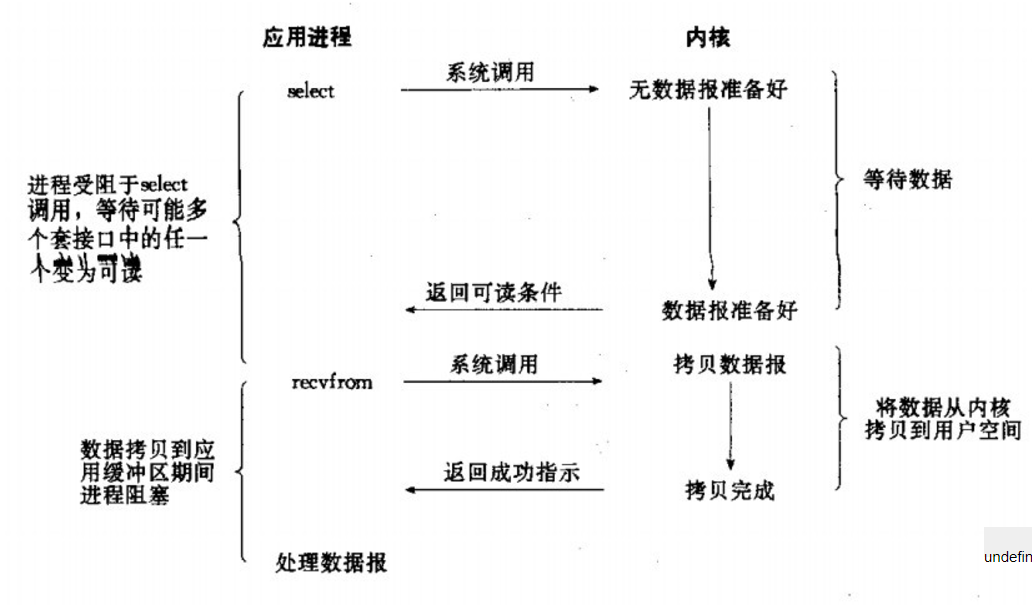
\includegraphics[width=0.5\textwidth]{img/select.png}
    \caption{select工作流程}
\end{figure}

select的工作流程:单个进程就可以同时处理多个网络连接的io请求(同时阻塞多个io操作)。基本原理就是程序呼叫select,然后整个程序就阻塞了,这时候,kernel就会轮询检查所有select负责的fd,当找到一个client中的数据准备好了,select就会返回,这个时候程序就会系统调用,将数据从kernel复制到进程缓冲区。

\subsubsection{poll简介}
poll的原理与select非常相似,差别如下:
\begin{itemize}
    \item 描述fd集合的方式不同,poll使用 pollfd 结构而不是select结构fd\_set结构,所以poll是链式的,没有最大连接数的限制;
    \item poll有一个特点是水平触发,也就是通知程序fd就绪后,这次没有被处理,那么下次poll的时候会再次通知同个fd已经就绪。
\end{itemize}

\subsubsection{epoll简介}
epoll在Linux2.6内核正式提出,是基于事件驱动的I/O方式,相对于select和poll来说,epoll没有描述符个数限制,使用一个文件描述符管理多个描述符,将用户关心的文件描述符的事件存放到内核的一个事件表中,这样在用户空间和内核空间的copy只需一次。优点如下:
\begin{enumerate}
    \item 没有最大并发连接的限制,能打开的fd上限远大于1024(1G的内存能监听约10万个端口)
    \item 采用回调的方式,效率提升。只有活跃可用的fd才会调用callback函数,也就是说 epoll 只管你“活跃”的连接,而跟连接总数无关,因此在实际的网络环境中,epoll的效率就会远远高于select和poll。
    \item 内存拷贝。使用mmap()文件映射内存来加速与内核空间的消息传递,减少复制开销。
\end{enumerate}

epoll对文件描述符的操作有两种模式:LT(level trigger,水平触发)和ET(edge trigger)。

\textbf{水平触发:}默认工作模式,即当epoll\_wait检测到某描述符事件就绪并通知应用程序时,应用程序可以不立即处理该事件;下次调用epoll\_wait时,会再次通知此事件。

\textbf{边缘触发:}当epoll\_wait检测到某描述符事件就绪并通知应用程序时,应用程序必须立即处理该事件。如果不处理,下次调用epoll\_wait时,不会再次通知此事件。(直到你做了某些操作导致该描述符变成未就绪状态了,也就是说边缘触发只在状态由未就绪变为就绪时通知一次)。

ET模式很大程度上减少了epoll事件的触发次数,因此效率比LT模式下高。

\subsection{HTTP重定向}
HTTP重定向响应报文状态码一般为3xx,这类状态码代表需要客户端采取进一步的操作才能完成请求。通常,这些状态码用来重定向,后续的请求地址(重定向目标)在本次响应的Location域中指明。

当且仅当后续的请求所使用的方法是GET或者HEAD时,用户浏览器才可以在没有用户介入的情况下自动提交所需要的后续请求。客户端应当自动监测无限循环重定向(例如:A→B→C→……→A或A→A),因为这会导致服务器和客户端大量不必要的资源消耗。按照HTTP/1.0版规范的建议,浏览器不应自动访问超过5次的重定向。

\subsubsection{300 Multiple Choices}
被请求的资源有一系列可供选择的回馈信息,每个都有自己特定的地址和浏览器驱动的商议信息。用户或浏览器能够自行选择一个首选的地址进行重定向。除非这是一个HEAD请求,否则该响应应当包括一个资源特性及地址的列表的实体,以便用户或浏览器从中选择最合适的重定向地址。这个实体的格式由Content-Type定义的格式所决定。浏览器可能根据响应的格式以及浏览器自身能力,自动作出最合适的选择。当然,RFC 2616规范并没有规定这样的自动选择该如何进行。如果服务器本身已经有了首选的回馈选择,那么在Location中应当指明这个回馈的URI;浏览器可能会将这个Location值作为自动重定向的地址。此外,除非额外指定,否则这个响应也是可缓存的。

\subsubsection{301 Moved Permanently}
被请求的资源已永久移动到新位置,并且将来任何对此资源的引用都应该使用本响应返回的若干个URI之一。如果可能,拥有链接编辑功能的客户端应当自动把请求的地址修改为从服务器反馈回来的地址。除非额外指定,否则这个响应也是可缓存的。新的永久性的URI应当在响应的Location域中返回。除非这是一个HEAD请求,否则响应的实体中应当包含指向新的URI的超链接及简短说明。如果这不是一个GET或者HEAD请求,那么浏览器禁止自动进行重定向,除非得到用户的确认,因为请求的条件可能因此发生变化。

\subsubsection{302 Found}
要求客户端执行临时重定向(原始描述短语为“Moved Temporarily”)。由于这样的重定向是临时的,客户端应当继续向原有地址发送以后的请求。只有在Cache-Control或Expires中进行了指定的情况下,这个响应才是可缓存的。新的临时性的URI应当在响应的Location域中返回。除非这是一个HEAD请求,否则响应的实体中应当包含指向新的URI的超链接及简短说明。如果这不是一个GET或者HEAD请求,那么浏览器禁止自动进行重定向,除非得到用户的确认,因为请求的条件可能因此发生变化。

\subsubsection{303 See Other}
对应当前请求的响应可以在另一个URI上被找到,当响应于POST(或PUT / DELETE)接收到响应时,客户端应该假定服务器已经收到数据,并且应该使用单独的GET消息发出重定向。这个方法的存在主要是为了允许由脚本激活的POST请求输出重定向到一个新的资源。这个新的URI不是原始资源的替代引用。同时,303响应禁止被缓存。当然,第二个请求(重定向)可能被缓存。新的URI应当在响应的Location域中返回。除非这是一个HEAD请求,否则响应的实体中应当包含指向新的URI的超链接及简短说明。

\subsubsection{304 Not Modified}
表示资源在由请求头中的If-Modified-Since或If-None-Match参数指定的这一版本之后,未曾被修改。在这种情况下,由于客户端仍然具有以前下载的副本,因此不需要重新传输资源。

\section{实验结果}
\subsection{实验环境}
本实验在Linux环境下使用python完成,主要使用python自带的socket库调用epoll函数处理客户端访问,主服务器维护各子服务器的状态,通过HTTP重定向将客户端请求分流到各个子服务器。

\subsection{结果展示}


\end{document}
